% !TEX root = ../main.tex

\chapter*{毕业设计（论文）中人工智能工具使用说明}
\addcontentsline{toc}{chapter}{人工智能工具使用说明}
\markboth{人工智能工具使用说明}{人工智能工具使用说明}

根据《上海交通大学关于在教育教学中使用 AI 的规范》以及本科毕业设计（论文）相关要求，本文对毕业设计（论文）完成过程中使用人工智能工具的情况说明如下。

\noindent\textbf{毕业设计（论文）标题：}基于 Flink 的动态 Kafka-Topic 发现与订阅机制研究

\noindent\textbf{学生姓名：}胡文杰\quad
\textbf{学号：}522031910511\quad
\textbf{指导教师：}任锐

\section*{一、本文使用的 AI 工具清单}
\addcontentsline{toc}{section}{一、本文使用的 AI 工具清单}

\begin{table}[H]
  \centering
  \caption*{本文使用的 AI 工具清单}
  \small
  \setlength{\tabcolsep}{4pt}
  \renewcommand{\arraystretch}{1.18}
  \begin{tabularx}{0.97\textwidth}{>{\centering\arraybackslash}p{0.07\textwidth}>{\raggedright\arraybackslash}p{0.18\textwidth}>{\raggedright\arraybackslash}p{0.15\textwidth}>{\raggedright\arraybackslash}p{0.18\textwidth}>{\raggedright\arraybackslash}X}
    \toprule
    序号 & AI 工具名称 & 版本/型号 & 应用部分 & 人为判断过程 \\
    \midrule
    1 & Cursor & GPT-5.5 & A2、C2、D1、D2、D3、E1、E2 &
    对 AI 给出的论文结构、文字表述、LaTeX 修改建议和代码审阅意见逐项人工核验；涉及技术结论时对照项目源码、Flink/Kafka 官方文档和本文实验记录进行检查；涉及格式修改时通过本地编译和 PDF 预览确认结果。 \\
    \bottomrule
  \end{tabularx}
\end{table}

\section*{二、应用部分对照表}
\addcontentsline{toc}{section}{二、应用部分对照表}

\begin{description}
  \item[A. 研究准备阶段] A1. 选题与方向设定；A2. 文献检索与筛选。
  \item[B. 研究设计阶段] B1. 研究思路设计；B2. 方法论构建；B3. 研究工具开发。
  \item[C. 研究实施阶段] C1. 实验/数据分析；C2. 代码编写与调试；C3. 数学建模与计算。
  \item[D. 论文写作阶段] D1. 大纲与逻辑优化；D2. 论文正文写作；D3. 语言与语法润色。
  \item[E. 其他辅助环节] E1. 参考文献与格式；E2. 图表/多媒体生成；E3. 学术反馈与模拟答辩。
\end{description}

\section*{三、使用说明}
\addcontentsline{toc}{section}{三、使用说明}

1. A2：在研究现状与相关技术整理过程中，AI 工具用于辅助梳理 Kafka、Flink、Kafka Connect、Debezium、Flink CDC 以及社区动态 Sink 提案之间的关系，并帮助形成对现有方案能力边界的归纳。相关内容由本人结合官方文档、开源项目资料和论文正文逻辑进行人工筛选与核验。

2. C2：在代码审阅和实验复现整理过程中，AI 工具用于辅助检查动态发现、route 映射、writer 生命周期、Checkpoint 协同和事务提交路径中可能影响论文论证的实现风险，并辅助整理实验运行命令。最终判断由本人结合项目源码、配置文件、编译结果和本地实验记录完成。

3. D1、D2、D3：在论文写作阶段，AI 工具用于辅助优化章节结构、增强需求分析与系统设计之间的衔接、润色中英文摘要和正文表述，并检查是否存在过于口语化或结论外推过度的表述。论文核心观点、章节取舍和最终文字均由本人确认。

4. E1、E2：在格式与图表整理过程中，AI 工具用于辅助检查参考文献格式、目录结构、表格排版、LaTeX 编译警告，以及使用 TikZ 绘制 route 生命周期状态图和 Exactly-once 提交流程序列图。所有格式修改均通过本地编译和 PDF 预览进行人工确认。

\section*{学术诚信声明}
\addcontentsline{toc}{section}{学术诚信声明}

本人承诺：论文核心观点、实验数据及结论均独立完成，AI 工具仅用于辅助性工作，已明确说明所有生成内容并在文中对应位置进行脚注标注。

\vspace{1.5em}

\begin{flushright}
  \begin{tabular}{l}
    承诺人：\raisebox{-0.45\height}{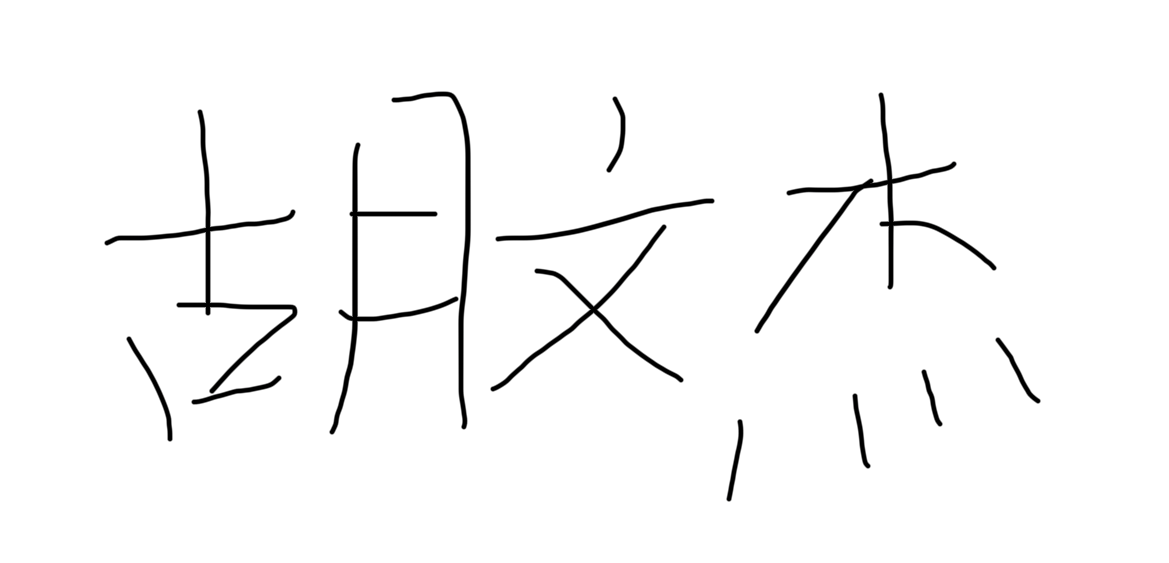
\includegraphics[height=1.0cm]{../my_signature.png}} \\
    日期：2026 年 5 月 8 日
  \end{tabular}
\end{flushright}
